\chapter{Gestión del Proyecto}\label{cap:gestion_proyecto}

\section{Tareas}\label{sec:tareas}

\subsubsection{T1: Estudio del estado del arte}\label{subsubsec:tareas_ob1}

\begin{itemize}[noitemsep]
      \item \textbf{T1.1: Revisión del estado del arte en entornos HPC} \\
            Estudiar la evolución histórica y tendencias actuales en la computación de alto rendimiento.

      \item \textbf{T1.2: Análisis del uso de contenedores en entornos HPC} \\
            Revisar tecnologías de contenedores aplicadas a entornos científicos y de alto rendimiento. Comparar contenedores frente a máquinas virtuales en cuanto a eficiencia, overhead y portabilidad en sistemas HPC.

      \item \textbf{T1.3: Estudio del uso de GPU en aplicaciones entornos HPC} \\
            Revisar el papel de las GPUs en la aceleración de aplicaciones científicas y de ingeniería. Identificar librerías y frameworks para programación en GPU. Analizar casos de éxito en la integración de GPU en entornos HPC.

      \item \textbf{T1.4: Investigación sobre el soporte de GPU en contenedores} \\
            Revisar soluciones actuales para ejecutar GPUs dentro de contenedores. Analizar el grado de compatibilidad con diferentes sistemas operativos y arquitecturas. Estudiar el impacto en rendimiento del uso de GPUs en entornos contenerizados en comparación con la ejecución nativa.
\end{itemize}

\subsubsection{T2: Diseño e implementación de la propuesta}\label{subsubsec:tareas_ob2}

\begin{itemize}[noitemsep]
      \item \textbf{T2.1: Selección de la aplicación o problema HPC a estudiar} \\
            Se seleccionará una aplicación representativa del ámbito HPC, justificando su elección en función de su relevancia científica, disponibilidad de código abierto y viabilidad técnica para su ejecución en diferentes plataformas y entornos contenerizados.

      \item \textbf{T2.2: Preparar entornos y dependencias} \\
            Se identificarán y documentarán las librerías y herramientas necesarias, incluyendo MPI, OpenMP y CUDA. Se garantizará la homogeneidad de las configuraciones en todos los sistemas de prueba y se detallarán los requisitos específicos para cada plataforma (Linux, Windows, macOS).

      \item \textbf{T2.3: Diseñar y construir imágenes de contenedor} \\
            Se desarrollarán Dockerfiles reproducibles que incluyan todas las dependencias necesarias, asegurando soporte para GPU mediante NVIDIA Container Toolkit. Las imágenes serán versionadas y almacenadas en un registro para facilitar su reutilización y trazabilidad.

      \item \textbf{T2.4: Definir casos de prueba y parámetros de ejecución} \\
            Se establecerán experimentos mononodo variando el número de hebras, experimentos multinodo con diferentes cantidades de nodos y casos combinados que exploren el espacio de parámetros hebras × nodos.

      \item \textbf{T2.5: Automatización y orquestación} \\
            Se implementarán scripts en para automatizar la ejecución de lotes de pruebas, así como la recogida y almacenamiento de logs y resultados.

      \item \textbf{T2.6: Instrumentación y métricas} \\
            Se instrumentará la aplicación para medir tiempos totales de ejecución, uso de CPU y otros recursos. Se calcularán métricas como aceleración, eficiencia, y \textit{overhead} comparando la ejecución en contenedor frente a la nativa. Se generarán gráficos comparativos para el análisis de resultados.

      \item \textbf{T2.7: Reproducibilidad y trazabilidad} \\
            Se mantendrá un repositorio con los Dockerfiles, scripts y documentación del proyecto. Se etiquetarán las versiones de las imágenes y dependencias para asegurar la reproducibilidad de los experimentos.
\end{itemize}

\subsubsection{T3: Evaluación de rendimiento}\label{subsubsec:tareas_ob3}

\begin{itemize}[noitemsep]
      \item \textbf{T3.1: Ejecución de pruebas comparativas} \\
            Se ejecutarán las mismas baterías de experimentos tanto en modo nativo como en contenedor. Se registrarán logs completos de cada ejecución.

      \item \textbf{T3.2: Recopilación y organización de resultados} \\
            Se guardarán los tiempos de ejecución y métricas de uso de recursos, clasificando los datos según plataforma (Linux, Windows y macOS) y tipo de acelerador (CPU y/o GPU). Se establecerá un formato homogéneo para los ficheros de resultados (CSV o base de datos).

      \item \textbf{T3.3: Visualización de resultados comparativos} \\
            Se generarán gráficos y tablas que destaquen los casos extremos (mejores y peores comportamientos), facilitando la interpretación de los resultados.
\end{itemize}

\subsubsection{T4: Análisis de resultados}\label{subsubsec:tareas_ob4}

\begin{itemize}[noitemsep]
      \item \textbf{T4.1: Revisión sistemática de los resultados experimentales} \\
            Se analizarán de manera estructurada los datos obtenidos en las pruebas, comparando el rendimiento entre ejecución nativa y contenerizada en las distintas plataformas (Linux, Windows y macOS) y ante el uso o no de aceleradores (CPU y/o GPU). Se identificarán tendencias generales, anomalías y comportamientos consistentes.

      \item \textbf{T4.2: Análisis cuantitativo del rendimiento} \\
            Se calcularán diferencias absolutas y relativas entre ejecución nativa y contenerizada, estimando overheads medios y por caso. Se evaluará la escalabilidad en cada escenario y se aplicará análisis estadístico para validar la significancia de las diferencias observadas.

      \item \textbf{T4.3: Análisis cualitativo} \\
            Se identificarán ventajas no estrictamente de rendimiento, como portabilidad, reproducibilidad y facilidad de despliegue, así como limitaciones observadas relacionadas con drivers de GPU, gestión de red en contenedores y problemas de compatibilidad.

      \item \textbf{T4.4: Detección de desafíos en la adopción de contenedores en entornos HPC} \\
            Se evaluará la complejidad asociada a la configuración, despliegue y mantenimiento de entornos contenerizados en sistemas HPC, incluyendo la integración de aceleradores como GPU y la gestión de dependencias específicas.

      \item \textbf{T4.5: Propuesta de líneas de investigación futura} \\
            A partir de los resultados y desafíos identificados, se propondrán posibles líneas de trabajo futuro.
\end{itemize}

\section{Planificación temporal}

En la tabla \ref{tab:planificacion-temporal} se presenta una estimación del tiempo necesario para completar cada una de las tareas principales del proyecto, desglosado en horas dedicadas por el desarrollador y el tutor.

\begin{table}[!ht]
      \centering
      \setlength{\tabcolsep}{3pt}
      \renewcommand{\arraystretch}{1.1}
      \begin{tabular}{|p{3cm}|r|r|}
            \hline
            \textbf{Tarea}  & \textbf{Desarrollador (h)} & \textbf{Tutor (h)} \\
            \hline
            Estado del arte & 50                         & 10                 \\
            Implementación  & 95                         & 8                  \\
            Evaluación      & 65                         & 7                  \\
            Análisis        & 40                         & 5                  \\
            \hline
            \textbf{Total}  & \textbf{250}               & \textbf{50}        \\
            \hline
      \end{tabular}
      \caption{Planificación temporal de tareas y horas estimadas}
      \label{tab:planificacion-temporal}
\end{table}

En la imagen \ref{fig:diagrama-gantt} se muestra un diagrama de Gantt que ilustra la distribución temporal de las tareas a lo largo del proyecto.

\begin{figure}[!h]
      \centering
      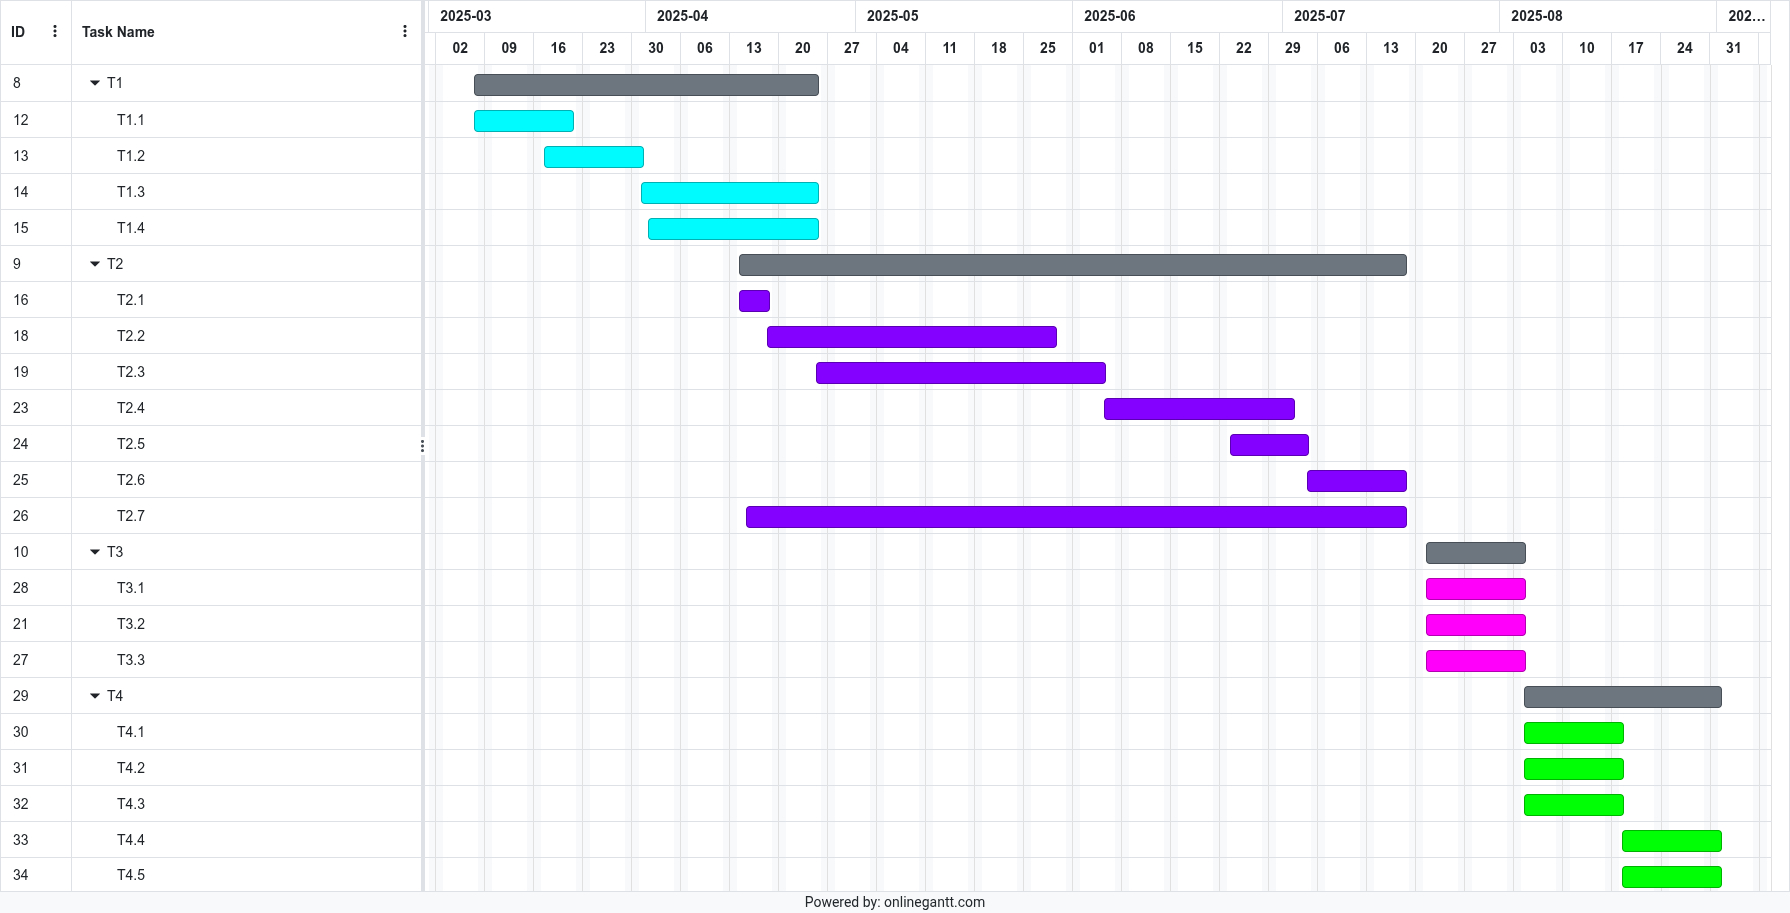
\includegraphics[width=\textwidth]{imagenes/cap2/diagrama_gantt.png}
      \caption{Diagrama de Gantt del proyecto realizado en Online Gantt\footnote{\url{https://www.onlinegantt.com/}}}
      \label{fig:diagrama-gantt}
\end{figure}

\section{Estimación de costes}

A continuación, se detallan los recursos necesarios para llevar a cabo el proyecto, incluyendo hardware, software y recursos humanos, junto con una estimación de los costes asociados.

\subsubsection{Hardware}

\begin{itemize}[noitemsep]
      \item Ordenador portátil LG Gram 14Z90Q-G.AA75B, este equipo se utilizará para el desarrollo general del trabajo: creación del código para las pruebas y creación de la memoria. Cuenta con un procesador Intel Core i7-1260P, 16 GB de RAM y 512 GB de almacenamiento SSD.

      \item Ordenador portátil Lenovo Legion 5, utilizado como plataforma principal para la ejecución de pruebas de rendimiento. Está equipado con un procesador AMD Ryzen 7 4800H (8 núcleos y 16 hilos), 16 GB de memoria RAM DDR4 y 512 GB de almacenamiento SSD NVMe. La presencia de la GPU NVIDIA permite la ejecución y evaluación de aplicaciones HPC que hacen uso de CUDA, así como la integración y validación del soporte de GPU en entornos contenerizados mediante NVIDIA Container Toolkit. Además, este equipo facilita la comparación de resultados entre ejecución nativa y contenerizada en escenarios reales de computación de alto rendimiento.

      \item Ordenador Apple Mac Mini M4, utilizado como plataforma de pruebas para la ejecución y validación de aplicaciones HPC en entornos macOS y arquitectura ARM. Este equipo incorpora un procesador Apple M4, 10 núcleos de CPU divididos en 4 de alto rendimiento y 6 de eficiencia, 10 núcleos de GPU integrada de última generación y 16 GB de memoria unificada. El Mac Mini M4 permitirá evaluar la compatibilidad y el rendimiento de contenedores en sistemas Apple Silicon.
\end{itemize}

\subsection{Recursos humanos}

\begin{table}[!ht]
      \centering
      \begin{tabular}{|l|l|r|}
            \hline
            \textbf{Dispositivo}   & \textbf{Descripción}             & \textbf{Coste (€)} \\
            \hline
            LG Gram 14Z90Q-G.AA75B & Portátil principal de desarrollo & 1\,000             \\
            Lenovo Legion 5        & Portátil de pruebas              & 500                \\
            Apple Mac Mini M4      & Dispositivo de pruebas Apple     & 599                \\
            \hline
            \textbf{Total}         &                                  & \textbf{2\,099}    \\
            \hline
      \end{tabular}
      \caption{Costes estimados de hardware para el proyecto}
      \label{tab:costes-hardware}
\end{table}

En la tabla \ref{tab:recursos-humanos} se detalla el coste por hora, las horas estimadas y el coste total de los recursos humanos necesarios para llevar a cabo el proyecto.

\begin{table}[!ht]
      \centering
      \begin{tabular}{|l|l|r|r|r|}
            \hline
            \textbf{Recurso}        & \textbf{Puesto}  & \textbf{€/h} & \textbf{Horas} & \textbf{Total (€)} \\
            \hline
            Fernando Cuesta Bueno   & Desarrollador    & 15           & 260            & 3\,750             \\
            Juan José Escobar Pérez & Tutor/Supervisor & 25           & 50             & 1\,750             \\
            \hline
            \textbf{Total}          &                  &              &                & \textbf{5\,500}    \\
            \hline
      \end{tabular}
      \caption{Costes estimados de recursos humanos para el proyecto}
      \label{tab:recursos-humanos}
\end{table}

El coste por hora del desarrollador ha sido obtenido a partir del salario medio por hora indicado en la página web \cite{joobleIngenieroInformatico}. Esta página recoge datos de diversas fuentes para calcular el salario medio en España para un ingeniero informático, que es de $17,98$€/h. Dado que el proyecto se realiza en el ámbito académico y no profesional, se ha estimado un coste por hora de $15$€/h para el desarrollador. Por otro lado, el coste por hora del tutor se ha estimado en $25$€/h, considerando su experiencia y rol de supervisión en el proyecto.

\subsection{Coste total del proyecto}

En el supuesto de que el proyecto se realizara en un entorno profesional, habría que considerar una cuota empresarial de un $30\%$ sobre el coste mostrado en la tabla \ref{tab:recursos-humanos}.

El coste total del proyecto se calcula sumando los costes de hardware y de recursos humanos. En la tabla \ref{tab:coste-total} se detalla el coste total estimado.

\begin{table}[!ht]
      \centering
      \begin{tabular}{|l|r|}
            \hline
            \textbf{Concepto} & \textbf{Coste (€)} \\
            \hline
            Hardware          & 2\,099             \\
            Recursos humanos  & 5\,500             \\
            Cuota empresarial & 1\,650             \\
            \hline
            \textbf{Total}    & \textbf{9\,249}    \\
            \hline
      \end{tabular}
      \caption{Coste total estimado del proyecto}
      \label{tab:coste-total}
\end{table}